%!TEX root = ../../main.tex

\section{Reduced Ordered Binary Decision Diagram} \label{sec:robdd}

In real-world cases, exploiting basic model checking algorithms is impossible due to the large amount of states to handle. 
In order to make them usable, we need adapt them by using Binary Decision Diagram which allows to represent and manipulate set of states, also called symbolic representation. 
They have been especially effective as algorithmic basis for symbolic model checkers.

Binary Decision Diagram (BDD) provides a data structure to represent and manipulate Boolean functions symbolically.
The Boolean formulas represented by BDDs are in If-then-else Normal Form (INF), that is a normal form where a formula can be either true, false or a if-then-else expression where the condition is a variable and the branches are formulas in INF. 
Another exploited tool is Shannon's expansion, useful to expand any Boolean functions. 
In our context, the expansion is interpreted as a if-then-else expression, where the condition is a variable $x$ and the co-factors being the branches.

\begin{definition}[If-then-else Normal Form (INF)]
The set of Boolean expressions in If-then-else Normal Form is defined by
\begin{flalign*}
t ::= 0 \; | \; 1 \; | \; x \to t_1,t_2 
\end{flalign*}
where $x$ is a variable.
\end{definition}

\begin{theorem}[\cite{principles-cps} Shannon's expansion]
For every Boolean expression $t$ and a variable $x$, $t \equiv x \to t[1/x],t[0/x]$.
Equivalently, we can express $t$ as $t \equiv (x \land t[1/x]) \lor (\neg x \land t[0/x]$ without using the if-then-else expression. Note that if $t$ has $k$ variables, then the two co-factors have $k-1$ variables.
\end{theorem}

Boolean expressions in INF can be viewed as binary graph known as decision diagram. Each internal node $v$ is labelled with a variable, retrievable by $var(v)$, and has two out-going edges: $low(v)$ to get the sub-tree root related to the negative co-factor and $high(v)$ to get the sub-tree root related to the positive co-factor.
There are three types of BDDs and one is the previous one but with a further condition. 
The first type is BDD, which is built by recursively applying Shannon's expansion on the branches until the branches has no variables. 
Note that BDD type impose no further rules, but it is just the diagram obtained by such procedure. 
One of the biggest issue with BDD is the non-canonicity, that is there could be two or more BDDs representing the same formula.
For this reason we require a BDD to be ordered, that is each sub-tree respects a linear ordering known a-priori. 
Then, to finally reach canonicity we require an Ordered BDD to be reduced, i.e. all nodes are unique (there are no two nodes such that they have the same variable, low and high values) and there are no redundancies (there are no nodes such that its low and high values are equals, and so it's useful). 
The chosen linear-ordering is very important because it could affect the size of the final ROBDD a lot.

\begin{definition}[\cite{principles-cps} Binary Decision Diagram (BDD)]
A BDD is a rooted and directed acyclic graph with: 
\begin{itemize}
    \item all non-terminals labelled with a Boolean variable;
    \item all terminals labelled with $0$ or $1$;
    \item all edged are labelled $0$ or $1$;
    \item all other internal nodes have out-degree two, with one outgoing edge called the low edge and the other called the high edge and are labelled with a variable. The two outgoing edges are given by two functions $low(u)$ and $high(u)$. 
\end{itemize}
\end{definition}

\begin{definition}[\cite{principles-cps} Ordered BDD (OBDD)]
A BDD is ordered if on all paths through the graph the variables respect a given linear order $x_1 < x_2 < \dots < x_n$.
\end{definition}

\begin{definition}[\cite{principles-cps} Reduced OBDD (ROBDD)]
A Ordered BDD is reduced if it's: unique, i.e. no two distinct internal nodes $u$ and $v$ have the same variable, low and high successor; non-redundant, i.e. no internal node $u$ has identical low and high successor.
\end{definition}

\begin{proposition}[\cite{principles-cps} Canonicity of ROBDD]
For a Boolean expression $t$ with variables $x_1 \dots x_n$ and a linear order $x_1 < \dots < x_n$, there exists a unique ROBDD that is equivalent to t.
\end{proposition}

\begin{figure}[!htp]
    \centering
    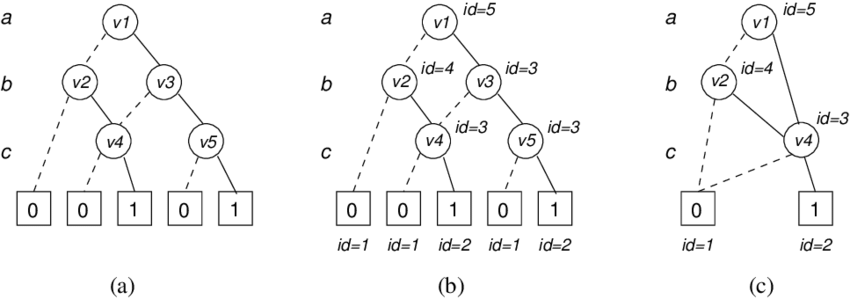
\includegraphics[width=0.8\linewidth]{figures/robdd-example.png}
    \caption{\cite{dhiraj-2023} Example of ROBDD construction for $f=(a \lor b) \land c$; a) OBDD for the variable order a,b,c; b) OBDD with unique identifiers; c) ROBDD for variable order a, b, c.}
    \label{fig:robdd-construction-example}
\end{figure}

From now on whenever it is written BDD, we mean ROBBD, because ROBDD are the only type of BDDs exploited in both practice and theory.
Since BDDs represent Boolean formulas, on them can be applied the common Boolean operations.
Given two BDDs $B_0$ and $B_1$ and denoting with $f(B_0)$ and $f(B_1)$ the two formulas represented by the two BDDs, the common Boolean operations that can be applied on them are:
\begin{itemize}
    \item $and(B_0,B_1)$, returning the ROBDD for the formula $f(B_0) \land f(B_1)$;
    \item $or(B_0,B_1)$, returning the ROBDD for the formula $f(B_0) \lor f(B_1)$;
    \item $not(B_0)$, returning the ROBDD for the formula $\neg f(B_0)$;
    \item $diff(B_0,B_1)$, returning the ROBDD for the formula $f(B_0) \land \neg f(B_1)$;
    \item $exists(B_0,X)$, returning the ROBDD for the formula $\exists X.f(B_0)$;
    \item $forall(B_0,X)$, returning the ROBDD for the formula $\forall X.f(B_0)$;
    \item $rename(B_0,X,Y)$, returning the ROBDD obtained by renaming variables in $X$ to $Y$;
    \item $restrict(B_0,X,1)$ and $restrict(B_0,X,0)$, returning the ROBDD for the formula $f(B_0)[1/X]$ and $f(B_0)[0/X]$, respectively the positive and negative co-factors.
\end{itemize} 

The complexity of each of the above operations is $O(\card{B_0})$ for unary ones and $O(\card{B_0} \cdot \card{B_1})$ for binary ones, with $\card{B}$ meaning the number of nodes of a given BDD $B$.

In order to apply BDDs to model checking, we need to interpret the whole state machine and sets of states as Boolean variables or Boolean formulas .
